
\chapter{Iterated Moore Equivalence}
\label{chap:imoore}

\section{Theory}
Standard Moore equivalence was created to minimize Moore automata in which the priority of every state matters; in other words, the occurrence set of a given run is considered. Parity automata on the other hand only use the smaller infinity set. The idea of the upcoming approach is to use this relaxation to give the standard Moore equivalence more freedom and remove additional states.

\begin{defn}
	Let $\mathcal{A} = (P, \Sigma, \delta, c)$ and $\mathcal{B} = (Q, \Sigma, \varepsilon, d)$ be DPAs and $S \subseteq P$. We say that \emph{$\mathcal{A}$ prepends $S$ to $\mathcal{B}$} if 
	\begin{itemize}
		\item $Q \cap S = \emptyset$
		\item $P = Q \cup S$
		\item $\delta\upharpoonright_{Q \times \Sigma} = \varepsilon$
		\item $c\upharpoonright_Q = d$
	\end{itemize}
	
	We assume $S$ to be an SCC in these use cases, i.e. from every $s \in S$, every other $s' \in S$ is reachable in $\mathcal{A}$.
\end{defn} 

\begin{defn}
\label{def:fwe:itmoore}
	Let $\mathcal{A} = (Q, \Sigma, \delta, c)$ be a DPA with SCCs $\mathcal{S} \subseteq 2^Q$. Let $\preceq \,\subseteq \mathcal{S} \times \mathcal{S}$ be a total preorder on the SCCs such that $S \preceq S'$ implies that $S'$ is reachable from $S$. For the $i$-th element w.r.t. this order, we write $S_i$, i.e. $S_0 \prec S_1 \prec \dots \prec S_{|\mathcal{S}|}$. 
	
	For every state $q$ in $\mathcal{A}$, let $\text{SCC}(q)$ be the SCC of $q$ and let $\text{SCCi}(q)$ be the index of that SCC, i.e. $\text{SCC}(q) = S_{\text{SCCi}(q)}$. Let $\preceq_Q \,\subseteq Q \times Q$ be a total preorder on the states such that $q \preceq_Q q'$ implies $\text{SCCi}(q) \leq \text{SCCi}(q')$.
	
	We inductively define a sequence of automata $(\mathcal{B}_i)_{0 \leq i \leq |\mathcal{S}|}$. For every $i$, we write $\mathcal{B}_i = (Q_i, \Sigma, \delta_i, c_i)$.
	
	\begin{itemize}
		\item The state sets are defined as $Q_i = \bigcup_{j=i}^{|\mathcal{S}|} S_j$.
		\item The base case is $\mathcal{B}_{|\mathcal{S}|} = \mathcal{A}\upharpoonright_{S_{|\mathcal{S}|}}$.
		\item Given that $\mathcal{B}_{i+1}$ is defined, let $\mathcal{B}'_i = (Q_i, \Sigma, q_0^{\prime i}, \delta_i, c'_i)$ be a DPA that prepends $S_i$ to $\mathcal{B}_{i+1}$ such that $\delta \upharpoonright_{Q_i \times \Sigma} = \delta_i$ and $c \upharpoonright_{S_i} = c'_i \upharpoonright_{S_i}$.
		\item Let $M'_i$ be the Moore equivalence on $\mathcal{B}'_i$. If $S_i = \{q\}$ is a trivial SCC, $q$ is not $M'_i$-equivalent to any other state, and there is a $p \in Q_{i+1}$ such that for all $a \in \Sigma$ $(\delta'_i(q, a), \delta'_i(p, a)) \in M'_i$, then let $p_0$ be $\preceq_Q$-maximal among those $p$ and let $c_i(r) = \begin{cases} c_{i+1}(p_0) & \text{if } r = q \\ c_{i+1}(r) & \text{else} \end{cases}$. If any of the three conditions is false, simply set $c_i = c'_i$.
	\end{itemize} 
	
	Let $M_i$ be the Moore equivalence on $\mathcal{B}_i$. We define $\equiv_{IM} \,:= M_0$ and call this the \emph{iterated Moore equivalence} of $\mathcal{A}$.
\end{defn}

At first, this definition might confuse when written down formally like this. We continuously add the SCCs of $\mathcal{A}$ starting from the \enquote{back}. In addition to computing the usual Moore equivalence on our automaton, we also take trivial SCCs into special consideration; as their priority cannot appear infinitely often on any run, its value is effectively arbitrary. We can therefore perform extra steps to more liberally merge it with other states.

The simple automaton in figure \ref{fig:fritzwilke:example} displays an example. We have $q_0 \not\equiv_M q_1$, as the two states have different priorities. With iterated Moore equivalence, we actually have $q_0 \equiv_{IM} q_1$:

First, we choose our order of SCCs as $S_0 = \{q_0\}$ and $S_1 = \{q_1\}$. $\mathcal{B}_1$ then has only one state $q_1$ with the transition to itself. $\mathcal{B}'_0$ is then the same automaton as $\mathcal{A}$. $S_0$ is a trivial SCC, it is not $M'_0$-equivalent to any other state and $(\delta'_0(q_0, a), \delta'_0(q_1, a)) \in M'_0$ for all $a$. Therefore, $c_0(q_0)$ is set to $1$ and we have $(q_0, q_1) \in M_0$.

\begin{figure}
\centering
\begin{tikzpicture}[shorten >=1pt,node distance=2cm,on grid,initial text=]
  \node[state]           (0)                {$q_0,0$};
  \node[state]           (1) [right=of 0]   {$q_1,1$};
  \path[->] (0) edge node [above] {a} (1)
            (1) edge [loop right] node [right] {a} (1);
\end{tikzpicture}
\caption{Example automaton to showcase iterated Moore equivalence.}
\label{fig:fritzwilke:example}
\end{figure}

\begin{defn}
	Let $\mathcal{A} = (Q, \Sigma, \delta, c)$ be a DPA. We define the \emph{iterated Moore merger function} $\mu_{IM} : \mathfrak{C}(\equiv_{IM}, \mathcal{A}) \rightarrow 2^Q$ as $\mu_{IM}(\kappa) = \{ q \in \kappa \mid q \text{ is } \preceq_\text{reach}^\mathcal{A} \text{-maximal in } \kappa \}$.
\end{defn}

\begin{theorem}
	Let $\mathcal{A}$ be a DPA and let $\mathcal{A}'$ be a representative merge of $\mathcal{A}$ w.r.t. $\mu_{IM}$. For all $q \in Q'$, $(\mathcal{A}, q) \equiv_L (\mathcal{A}', q)$.
\end{theorem}

\begin{proof}
	By definition of the iterated Moore equivalence, we only have $c(p) \neq c'(p)$ if $\{p\}$ is a trivial SCC in $\mathcal{A}$. By having candidates of the merge be $\preceq_\text{reach}^\mathcal{A}$-maximal, we assure that for all chosen representatives $r_\kappa$, $c(r_\kappa) = c_{|\mathcal{S}|}(r_\kappa)$. With Lemma \ref{lem:general:trivial_scc_dont_matter}, this finishes our proof.
\end{proof}

\vspace{10pt}

Unfortunately, we were not able to find or prove any relation between iterated Moore equivalence and other relations we established so far. We therefore end this section with two open questions.

\begin{itemize}
	\item Is $|\mathfrak{C}(\equiv_M, \mathcal{A})| \geq |\mathfrak{C}(\equiv_{IM}, \mathcal{A})|$ true for all $\mathcal{A}$?
	\item If $\mathcal{A}$ is $c$-normalized, what is the relation between $\equiv_{IM}$ and $\equiv_\text{de}$?
\end{itemize}


\section{Computation}
\begin{lem}
	For a given DPA $\mathcal{A}$, $\mu_{IM}$ can be computed in $\mathcal{O}(|\mathcal{S}| \cdot |Q| \cdot \log |Q|)$.
\end{lem}

\begin{proof}
	$\equiv_{IM}$ is already basically defined as an algorithm. We use $|\mathcal{S}|$ many steps of computing Moore equivalence and then checking whether the priority of the newly added state should be changed. The first can be done in log-linear time (Corollary \ref{cor:general:M_loglin}), the second in linear time. This gives us a runtime of $\mathcal{O}(|\mathcal{S}| \cdot |Q| \cdot \log |Q|)$ to calculate $\equiv_{IM}$.

	To build $\mu_{IM}$ from that can be done in linear time by Lemma \ref{lem:general:reach_topo_lintime}.
\end{proof}


\section{Efficiency}
Figure \ref{fig:imoore:empirical_size_hist} shows that the iterated Moore merger actually performs a decent job at reducing the number of states in \textsf{detspot} and \textsf{detnbaut}, even when compared to the normal Moore merger in figure \ref{fig:general:empirical_moore_size_hist}. However, the absolute number of removed states actually stays rather low and consequently the automata that witness a large relative reduction have a small number of states to begin with. This can be seen in figure \ref{fig:imoore:empirical_reduct_abs}: \textsf{detnbaut} rarely has more than 10 states removed, and \textsf{detspot} stays within a similar range of reduction as figure \ref{fig:general:empirical_moore_reduct_abs}, with the exception of a few outliers.

This result is to be expected. As figure \ref{fig:rawstats:rawstats_sccs} showed, very few automata contain more than five SCCs. The iterated Moore procedure can only exceed the normal Moore quotient by using trivial SCCs.

As predicted by the theoretical complexity of the algorithm, figure \ref{fig:imoore:empirical_time} confirms that the iterated Moore merger is fast to apply, only reaching a run time of one second at 200 states.


\begin{figure}
	\centering
	\begin{minipage}{0.49\textwidth}
		\includegraphics[page=6,height=.3\textheight]{../data/analysis/iterated_moore/gendet_ap1.pdf} 
		\includegraphics[page=6,height=.3\textheight]{../data/analysis/iterated_moore/detspot_ap1.pdf} 
		\includegraphics[page=6,height=.3\textheight]{../data/analysis/iterated_moore/detnbaut_ap1.pdf} 
		\caption{State reduction of different automata using $\mu_{IM}$.}
		\label{fig:imoore:empirical_size_hist}
	\end{minipage}
	\hfill
	\begin{minipage}{0.49\textwidth}
		\includegraphics[page=2,height=.3\textheight]{../data/analysis/iterated_moore/gendet_ap1.pdf} 
		\includegraphics[page=2,height=.3\textheight]{../data/analysis/iterated_moore/detspot_ap1.pdf} 
		\includegraphics[page=2,height=.3\textheight]{../data/analysis/iterated_moore/detnbaut_ap1.pdf} 
		\caption{State reduction of different automata using $\mu_{IM}$.}
		\label{fig:imoore:empirical_reduct_abs}
	\end{minipage}
\end{figure}


\begin{figure}
	\centering
	\begin{minipage}{0.49\textwidth}
		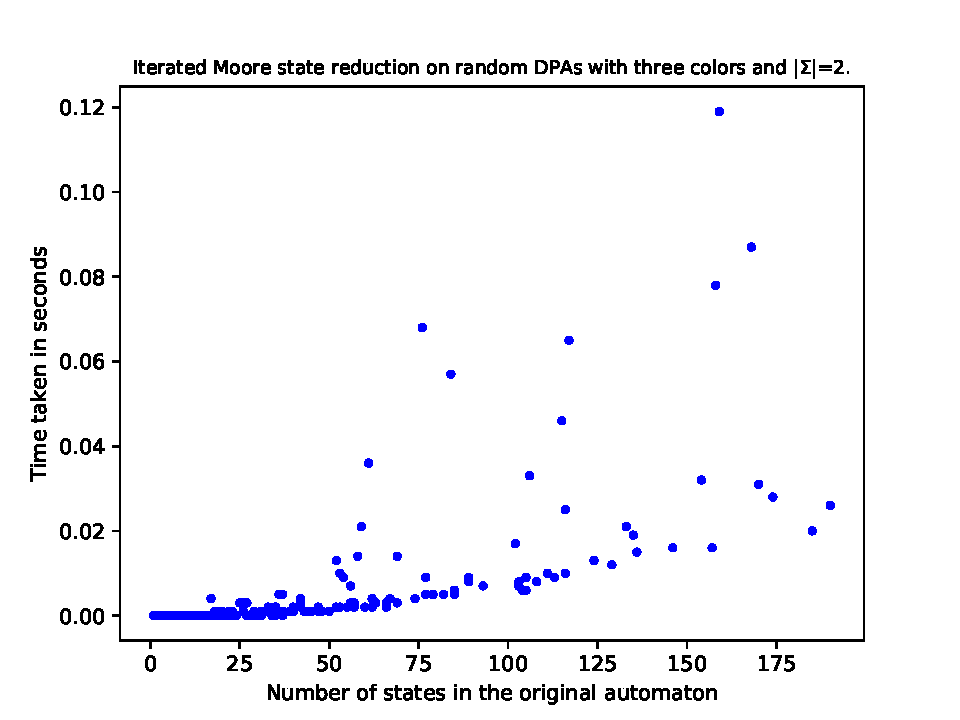
\includegraphics[page=1,height=.3\textheight]{../data/analysis/iterated_moore/gendet_ap1.pdf} 
		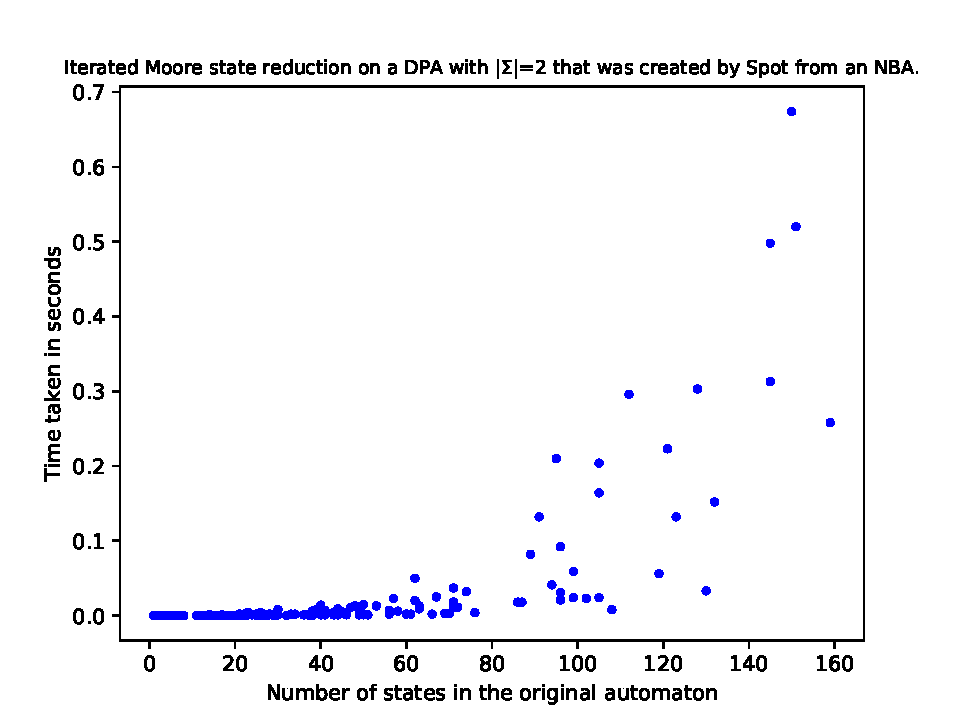
\includegraphics[page=1,height=.3\textheight]{../data/analysis/iterated_moore/detspot_ap1.pdf} 
		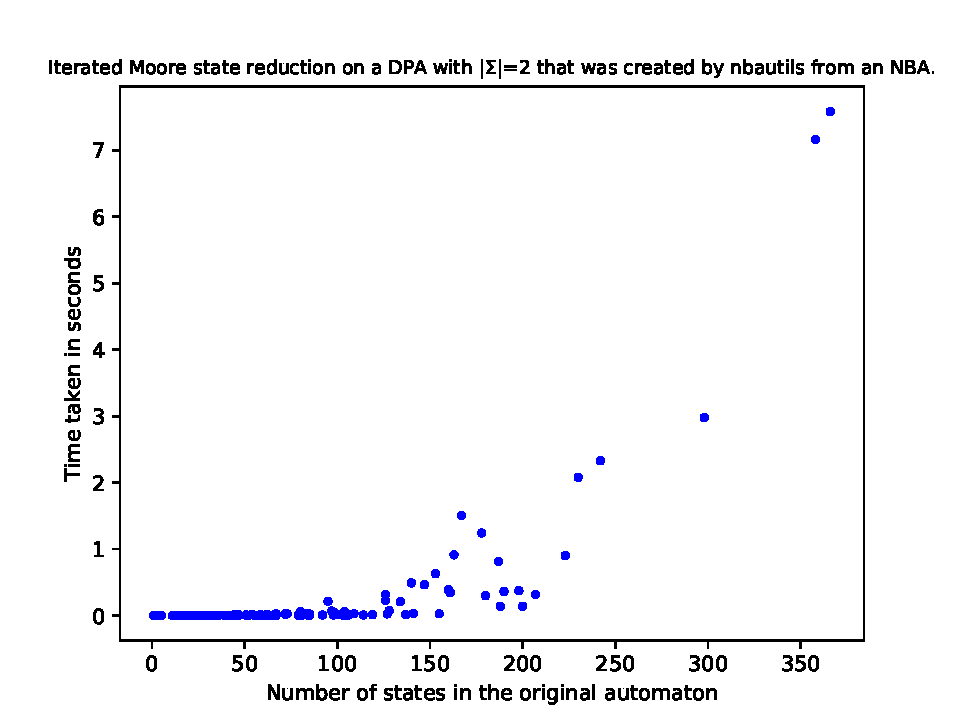
\includegraphics[page=1,height=.3\textheight]{../data/analysis/iterated_moore/detnbaut_ap1.pdf} 
		\caption{Run time of the state reduction of different automata using $\mu_{IM}$.}
		\label{fig:imoore:empirical_time}
	\end{minipage}
\end{figure}


